\documentclass[12pt,notitlepage]{article}

\usepackage[utf8]{inputenc}
\usepackage[english]{babel}

\usepackage{upgreek}

% https://tex.stackexchange.com/questions/11778/modifying-everydisplay-causes-the-align-environment-to-stop-working
\let\displaystyle\textstyle


%
\usepackage[
backend=biber,
%
style=alphabetic, % [GSR03]
% style=nature, % [1]
%
giveninits=true,
url=false,
isbn=false,
backref=true,
sorting=ynt,
block=none,
maxcitenames=3,
maxbibnames=100,
]{biblatex}
%
% https://tex.stackexchange.com/questions/20335/proper-casing-in-citation-bibliography-titles-using-biblatex-biber
%\DeclareFieldFormat{titlecase}{\MakeSentenceCase*{#1}}
%
\addbibresource{refs.bib}


\usepackage{amsmath, amsfonts, amssymb, mathtools}
\usepackage[svgnames]{xcolor}
\usepackage{datetime2}
\usepackage[
	colorlinks=true, 
	citecolor={DarkRed}, urlcolor={DarkBlue}, linkcolor={DarkBlue},
]{hyperref}


% https://tex.stackexchange.com/questions/3802/how-to-get-doi-links-in-bibliography
% \usepackage{doi}

% 
\usepackage[version=4]{mhchem}
\mhchemoptions{font=sf}

% http://mirrors.ibiblio.org/CTAN/macros/latex/contrib/siunitx/siunitx.pdf
\usepackage{siunitx}


\usepackage{fullpage}

% Paragraph spacing
\usepackage{parskip}
%\usepackage{enumitem}

\usepackage{xspace}

\usepackage{graphicx}
\graphicspath{{../code/}{../images/}}
\DeclareGraphicsExtensions{.pdf,.eps,.png}

% https://tex.stackexchange.com/questions/202046/width-of-the-caption-of-a-figure
% https://tex.stackexchange.com/questions/29039/how-to-limit-the-figure-caption-width
% https://tex.stackexchange.com/questions/822/change-the-font-of-figure-captions
\usepackage[margin=10px,font={small}]{caption}
% https://tex.stackexchange.com/questions/25879/multiple-captions-for-a-single-figure
\usepackage{subcaption}


% http://www.texfaq.org/FAQ-ftnsect
\usepackage[stable]{footmisc}

% https://tex.stackexchange.com/questions/20792/how-to-superimpose-latex-on-a-picture
\usepackage[percent]{overpic}

%\usepackage{epstopdf}

% Tables (the order matters here)
\usepackage{makecell}
\usepackage{booktabs}
\usepackage{arydshln}

% https://tex.stackexchange.com/questions/109467/footnote-in-tabular-environment
\usepackage{footnote}
\makesavenoteenv{tabular}
\makesavenoteenv{table}

% https://tex.stackexchange.com/questions/66896/ref-chapter-name-in-latex
\usepackage{nameref}


% https://tex.stackexchange.com/questions/10130/use-the-values-of-title-author-and-date-on-a-custom-title-page
\usepackage{authoraftertitle}

% https://en.wikibooks.org/wiki/LaTeX/Footnotes_and_Margin_Notes#Margin_Notes
\usepackage{marginnote}

% For editing purposes:
%\usepackage[margin=10pt]{geometry}

% https://latex.org/forum/viewtopic.php?t=10456
\usepackage{titlesec}
\titleformat{\subsubsection}[runin]% runin puts it in the same paragraph
{\normalfont\bfseries}% formatting commands to apply to the whole heading
{\thesubsubsection}% the label and number
{}% space between label/number and subsection title
{}% formatting commands applied just to subsection title
[.]% punctuation or other commands following subsection title



% https://bitbucket.org/goodnightmath/covariance/src/master/tex/main.tex

%%%%%%%%%%%%%%%%%%%%%%%%%%%%%%%%%%%%%%%%%%%%%%%%%%%%%%%%%%%%%%%%%%%%%%%%%%%%%%%
\providecommand{\TODO}[1]{\textrm{\color{red}TODO: #1}}

% http://tex.stackexchange.com/a/106577/44073
\usepackage{ifthen}
\newcounter{todoindex}\setcounter{todoindex}{0}
\newcommand\ADDTODO[1]{%
	\addtocounter{todoindex}{1}%
	\expandafter\gdef\csname todo\roman{todoindex}\endcsname{#1}%
	%\expandafter\csname todolabel\roman{todoindex}\endcsname
	\label{todolabel\roman{todoindex}}
}
\renewcommand\TODO[1]{%
	{%
		\ADDTODO{#1}%
		{\textrm{\color{red}TODO(\arabic{todoindex}): #1}}%
	}%
}
\newcommand\CHECK[1]{%
	\ADDTODO{CHECK CLAIM: {#1}}%
	{\color{toverify}#1}%
	\smash{\marginnote{\text{\color{red}*}}}%
}
\newcounter{indextodo}
\newcommand{\SHOWTODOS}{%
	\setcounter{indextodo}{0}%
	\begin{enumerate}
	\item[{\color{red} TODOs:}]
	\whiledo{\value{indextodo} < \value{todoindex}}{%
		\addtocounter{indextodo}{1}%
		\item[\color{red}\arabic{indextodo}.]
		p.\pageref{todolabel\roman{indextodo}}.
		%
		\csname todo\roman{indextodo}\endcsname
	}%
	\end{enumerate}
}
%%%%%%%%%%%%%%%%%%%%%%%%%%%%%%%%%%%%%%%%%%%%%%%%%%%%%%%%%%%%%%%%%%%%%%%%%%%%%%%


%%%%%%%%%%%%%%%%%%%%%%%%%%%%%%%%%%%%%%%%%%%%%%%%%%%%%%%%%%%%%%%%%%%%%%%%%%%%%%%
\providecommand{\CODE}[1]{\href{#1}{code}}
\providecommand{\SHOWCODES}{}

\newcommand\codeprefix{https://github.com/numpde/nct1/tree/}

% http://tex.stackexchange.com/a/10657\texttt{7/44073
\usepackage{ifthen}
\newcounter{codeindex}\setcounter{codeindex}{0}
\newcommand\ADDCODE[1]{%
	\addtocounter{codeindex}{1}%
	\expandafter\gdef\csname code\roman{codeindex}\endcsname{#1}%
	\label{codelabel\roman{codeindex}}%
}
\renewcommand\CODE[1]{%
	{%
		\ADDCODE{\href{\codeprefix#1}{\texttt{#1}}}%
		{\href{\codeprefix#1}{\#\arabic{codeindex}}}%
	}%
}
\newcount\fooo
\newcounter{indexcode}
\long\def\addto#1#2{\expandafter\def\expandafter#1\expandafter{#1#2}}
\renewcommand{\SHOWCODES}{%
	\def\tabledata{}
	\setcounter{indexcode}{0}%
	\fooo=0\loop\advance\fooo+1
		\addto\tabledata{%
			\addtocounter{indexcode}{1}%
			\#\arabic{indexcode} &
			p.\pageref{codelabel\roman{indexcode}} &
			\csname code\roman{indexcode}\endcsname \\ 
		}
	\ifnum \fooo < \thecodeindex
	\repeat
	
	\begin{tabular}{c|c|c}
		 & page & \url{\codeprefix} ... \\
		\hline
		\tabledata
	\end{tabular}
}
%%%%%%%%%%%%%%%%%%%%%%%%%%%%%%%%%%%%%%%%%%%%%%%%%%%%%%%%%%%%%%%%%%%%%%%%%%%%%%%




\renewcommand{\d}{\mathrm{d}}
\newcommand{\ddt}{\frac{\d}{\d{t}}}

\newcommand{\TEXT}[1]{\quad\text{#1}\quad}
\newcommand{\with}{\text{$\,{:}\,$}}

\newcommand{\cbra}[1]{{\ensuremath{\color{gray}{#1}}}}
\newcommand{\signal}[1]{{{\cbra{\langle}\ce{#1}\cbra{\rangle}}}}
\newcommand{\protein}[1]{{{\cbra{(}\ce{#1}\cbra{)}}}}
\newcommand{\promoter}[1]{{{\cbra{[}\ce{#1}\cbra{]}}}}

% https://tex.stackexchange.com/questions/543953/arrow-with-blunted-end-head-in-math-mode
\newcommand{\act}{\ {\ensuremath{\mathbin{\to}}}\ }
\newcommand{\rep}{\ {\ensuremath{\mathrel{\raisebox{-.3ex}{\rotatebox{90}{\scalebox{1}[1.2]{$\bot$}}}}}}\ }

\def\[#1\]{\begin{align}#1\end{align}}

% https://tex.stackexchange.com/questions/114113/how-to-label-text-with-equation-number
\newcommand{\eqnum}{\leavevmode\hfill\refstepcounter{equation}\textup{{(\theequation)}}}

\newcommand{\starlink}[1]{\textsuperscript{\makebox[0pt]{\href{#1}{\color{white}$\star$}}}}

\newcommand{\hh}[1]{{\color{Purple}#1}}
\newcommand{\ra}[1]{{\color{Blue}#1}\marginnote{\TODO{review}}}

%

\title{%
A minimalistic computational model of NCT%
\thanks{%
R.~Andreev, L.~Kapinos, and R.~Y.~H.~Lim.
\today
\hfill
\tiny\color{lightgray}\hfill{\DTMnow}
}}

\date{}
\newcommand{\linktodoc}{http://bit.ly/}



\begin{document}



\maketitle

{
\small
\textbf{Abstract}.
%
We develop a minimalistic computational
model of 
NCT
that mimics
the live cell and (more closely) the artificial cell.
%
%
We are particularly
interested in 
the nuclear-to-cytoplasmic contrast
of 
certain molecular species,
at steady state,
namely,
RanGTP,
transport receptors,
and
cargo,
since these can be measured in experiments.
}


{
\small
\textbf{Abbreviations}.
%
NCT = nucleocytoplasmic transport;
NPC = nuclear pore complex;
NE = nuclear envelope;
IBB = importin beta binding; 
ODE = ordinary differential equations;
FG-nups = FG-nucleoporins;
SPR = surface plasmon resonance;
N:C = nuclear-to-cytoplasmic.
}

\section{Introduction}

%

The base layer of NCT is the establishment of 
the RanGTP gradient
for which we use the ``minimal Ran gradient system''
of \cite{GoerlichSeewaldRibbeck2003};
see \S\ref{s:GSR03:Ran}.
%
%
Still following \cite{GoerlichSeewaldRibbeck2003},
we add importin-mediated transport 
for IBB cargos.
%
i.e.~cargos that do not require an adapter.
%
%
%
In this model,
the nuclear pore is chemically inert 
and only serves as a diffusion channel,
but in the cell this is not the case.
%
To model that,
we first abstract
the base layer into a single
Ran gradient pump characterized
by a single rate, Eqn.~\ref{e:pump}. 

%

In \S\ref{ss:ranbp1} we take a look at the role
of RanBP1
in the hydrolysis of RanGTP
and associated species
but
for simplicity
abstract this process into 
one hydrolysis rate, Eqn.~\eqref{e:hydrolysis}.

%

Finally, in \S\ref{ss:3s}
we develop 
a computational model
that focuses
on the main players of NCT,
that is
{RanGTP},
{Imp$\upbeta$} (karyopherin-beta),
{Imp$\upalpha$} (karyopherin-alpha),
{CAS} (exportin),
{NLS} (cargo)
and
the nuclear pore itself.
%
%
%
In this model,
any species transits the NPC
in these steps:
binding to one side of the pore,
passing into the pore channel,
binding to the other side,
and unbinding on the other side.
%
%
This allows us
to reproduce the accumulation
of transport receptors
inside the NPC.

% Note: ImpBeta = KapBeta1

Each computational model is formulated as an ODE
in MATLAB/SimBiology.
%
In addition to kinetic parameters
this requires the initial concentrations of all chemical species.
%
We compute the ODE numerically until steady state
and report the final concentrations
in nucleus, cytoplasm and at the nuclear envelope, where applicable.



\section{NCT models}

\subsection{GSR'03 model of NCT} \label{s:GSR03}

\subsubsection*{Ran gradient} \label{s:GSR03:Ran}

The Ran gradient,
i.e.~the nuclear accumulation of \ce{Ran.GTP},
is the base layer of nucleocytoplasmic transport.
%
%
We implement it as
the ``minimal Ran gradient system'' from 
\cite{GoerlichSeewaldRibbeck2003}.
%
%
The equations are recapitulated in
\S\ref{s:app:gsr-ran}
and
the constants are collected in 
Table~\ref{t:GSR-const}.
%
%
This gradient
can be harnessed
by converting nuclear \ce{Ran.GTP} back to cytoplasmic \ce{Ran.GDP}.
%
For this reason,
\cite{GoerlichSeewaldRibbeck2003}
introduced
the ``dynamic capacity'' \ce{Ex}
as the maximal possible steady-state (positive) flux
of nuclear \ce{Ran.GTP} to cytoplasmic \ce{Ran.GDP}.
%
We determine it using the additional equation \eqref{e:Ex}.

%

The fluxes 
are in units of concentration/time (\si{\micro M \per s}).
%
The ones across the nuclear boundary
have positive sign when exiting the nucleus
and are normalized to the nuclear volume.
%
Thus,
the \emph{amount} exiting the nucleus per unit of time is
$\ce{flux} \times V_\text{nuc}$.

%

Simulating the ODE
across the scenarios of 
\cite{GoerlichSeewaldRibbeck2003}
we obtain 
results that are sufficiently close
to the original,
see Table~\ref{t:GSR-Ran-Runs}.
%
%
Importantly,
an order of 1000-fold nuclear enrichment of \ce{Ran.GTP}
is sustained in steady-state.
%
Moreover, the dynamic capacity clocks in at around
$
	\SI{0.6}{\micro M / s}
$
in most cases,
meaning the Ran gradient is established within seconds.
%
%
Therefore,
we will replace the whole Ran gradient layer
by a virtual pump
\[
	\label{e:pump}
	%
	\text{cytoplasmic \ce{Ran . GDP}} 
	\ce{->}
	\text{nuclear \ce{Ran . GTP}} 
	\TEXT{with kinetic rate \SI{0.1}{s^{-1}}.}
\]
%
%
This rate is chosen conservatively
(a concentration of $\SI{1}{\micro M}$ of cytoplasmic \ce{Ran . GDP} generates
a flux of $\SI{0.1}{\micro M / s}$)
but 
it will be
sufficient for our purposes.
%
%
%
See Code \CODE{main/code/20210225-GSR/v1}.

%

\subsubsection*{Coupling of importin-mediated transport} \label{s:GSR03:Imp}

A coupling of the Ran gradient
to 
importin--cargo transport
was proposed in 
\cite[\href{https://i.ibb.co/yY816bj/Goerlich-Seewald-Ribbeck-2003-Fig6-A.png}{Fig.~6A}]{GoerlichSeewaldRibbeck2003}.
%
This model thus includes
kinetics of \ce{Imp$\upbeta$} and IBB cargo,
in addition to the Ran gradient.
%
%
Few details were provided in \cite{GoerlichSeewaldRibbeck2003},
so we formulate a version of it here explicitly.
%
%
The following equations
comprise
the handling of cargo by \ce{Imp$\upbeta$} in the cytoplasm,
%
%
\begin{subequations}
\[
	\label{e:v2-1}
	%
	\ddt
	[\ce{Imp\beta . Ran . GTP}]_\text{cyt}
	& = 
	-
	\ce{R_{cyt}}
	+
	\ce{F_{\ce{Imp\beta . Ran . GTP}}}
	\frac{V_\text{nuc}}{V_\text{cyt}} 
	-
	\ce{GAP_{{Imp\beta}}}
	+
	\ce{Knockoff_{cyt}}
	%
	\\
	\label{e:v2-2}
	%
	\ddt
	[\ce{Imp\beta}]_\text{cyt}
	& = 
	%
	+
	\ce{R_{cyt}} + \ce{C_{cyt}}
	+
	\ce{F_{\ce{Imp\beta}}}
	\frac{V_\text{nuc}}{V_\text{cyt}} 
	+
	\ce{GAP_{{Imp\beta}}}
	%
	\\
	\label{e:v2-3}
	%
	\ddt
	[\ce{Imp\beta . Cargo}]_\text{cyt}
	& = 
	-
	\ce{C_{cyt}}
	+
	\ce{F_{\ce{Imp\beta . Cargo}}} \frac{V_\text{nuc}}{V_\text{cyt}}
	-
	\ce{Knockoff_{cyt}}
	%
	\\
	\label{e:v2-4}
	%
	\ddt
	[\ce{Cargo}]_\text{cyt}
	& = 
	+
	\ce{C_{cyt}}
	+
	\ce{F_{\ce{Cargo}}} \frac{V_\text{nuc}}{V_\text{cyt}}
	+
	\ce{Knockoff_{cyt}}
\]
\end{subequations}
%
with the fluxes
%
\begin{subequations}
\[
	%
	\label{e:v2-R}
	%
	\ce{R_{cyt}}
	& :=
	-
	k_\text{on}^\text{R} [\ce{Imp\beta}] [\ce{Ran . GTP}]_\text{cyt}
	+
	k_\text{off}^\text{R} [\ce{Imp\beta . Ran . GTP}]_\text{cyt}
	%
	\\
	\label{e:v2-C}
	%
	\ce{C_{cyt}}
	& :=
	-
	k_\text{on}^\text{C}
	[\ce{Imp\beta}]
	[\ce{Cargo}]_\text{cyt}
	%\qquad
	+
	k_\text{off}^\text{C}
	[\ce{Imp\beta . Cargo}]_\text{cyt}
	.
\]
\end{subequations}
%
%
%
The forward flux of the reaction
\[
	\label{e:knockoff}
	\ce{Imp\beta . Cargo + \ce{Ran . {GTP}} <=>> Imp\beta . \ce{Ran . {GTP}} + Cargo}
\]
is called \ce{Knockoff}.
%
It is modeled as a one-way reaction
with forward rate $k_\text{knockoff}$.
%
%
%
The GSR equations are modified accordingly:
%
\[
	\label{e:Eq1'}
	\tag{\ref{e:Eq1}$'$}
	%
	\ddt
	[\ce{Ran.GDP}]_\text{cyt}
	& =
	\eqref{e:Eq1} + \ce{GAP_{{Imp\beta}}}
	%
	\\
	\label{e:Eq2'}
	\tag{\ref{e:Eq2}$'$}
	%
	\ddt
	[\ce{Ran.GTP}]_\text{cyt}
	& = 
	\eqref{e:Eq2} + \ce{R_{cyt}} - \ce{Knockoff_{cyt}}
\]
%
%
Analogous nuclear equations
(without \ce{GAP}) 
are implemented, but are omitted here.
%
Analogously to \eqref{e:Eq11}/\eqref{e:Eq12}
we have 
the additional nuclear-to-cytoplasmic diffusion fluxes
%
\[
	\label{e:F4}
	%
	\ce{F_{\ce{Imp\beta . Ran . GTP}}},
	\quad
	\ce{F_{\ce{Imp\beta}}},
	\quad
	\ce{F_{\ce{Imp\beta . Cargo}}},
	\quad
	\ce{F_{\ce{Cargo}}}
\]
with the permeability constants
given in
Table~\ref{t:GSR-ImpB-const}.

%

SPR experiments of \cite{Catimel2001}
indicated that
the IBB domain of importin-$\alpha$ 
%(\TODO{fused to ?})
binds importin-$\beta$
and undergoes a conformational change,
\[
	\label{e:A*B}
	%
	\ce{A + B \rightleftharpoons AB \rightleftharpoons A^*B}
	.
\]
%
We therefore assume the analogous reaction
\[
	\label{e:Cargo*B}
	%
	\ce{
		{Cargo} + {Imp\beta}
		<=>[k_{a1}][k_{d1}]
		Cargo . {Imp\beta}
		<=>[k_{a2}][k_{d2}]
		Cargo^* . {Imp\beta}
	}
	.
\]
%
%
Examples of the kinetic constants
are available in \cite[Table~I]{Catimel2001},
e.g.,
\[
	\label{e:k-A*B}
	%
	k_{a1} = \SI{0.11}{\micro M^{-1} . s^{-1}},
	\quad
	k_{d1} = \SI{0.024}{s^{-1}},
	\qquad
	k_{a2} = \SI{0.024}{s^{-1}},
	\quad
	k_{d2} = \SI{7.4e-4}{s^{-1}},
\]
for an IBB domain binding to \ce{Imp\beta}.
%
%
The intermediate state in \eqref{e:A*B} is transient
on a moderately relevant time-scale
%see Fig.~\ref{f:A*B}
(Code \protect\CODE{main/code/20210407-Rearrangement}).
%
Therefore,
here we lump the complexed states together
and take
$k_\text{on}^\text{C} := k_{a1}$ and 
$k_\text{off}^\text{C} := k_{d1} \frac{k_{d2}}{k_{a2} + k_{d2}}$
as the effective kinetic rates 
for \eqref{e:v2-C}, cf.~Table~\ref{t:GSR-ImpB-const}.
%
% LK: 
%	          kd1 kd2
%	KD = -----------------
%	      (ka2 + kd2) ka1
%


%\begin{figure}
%\centering
%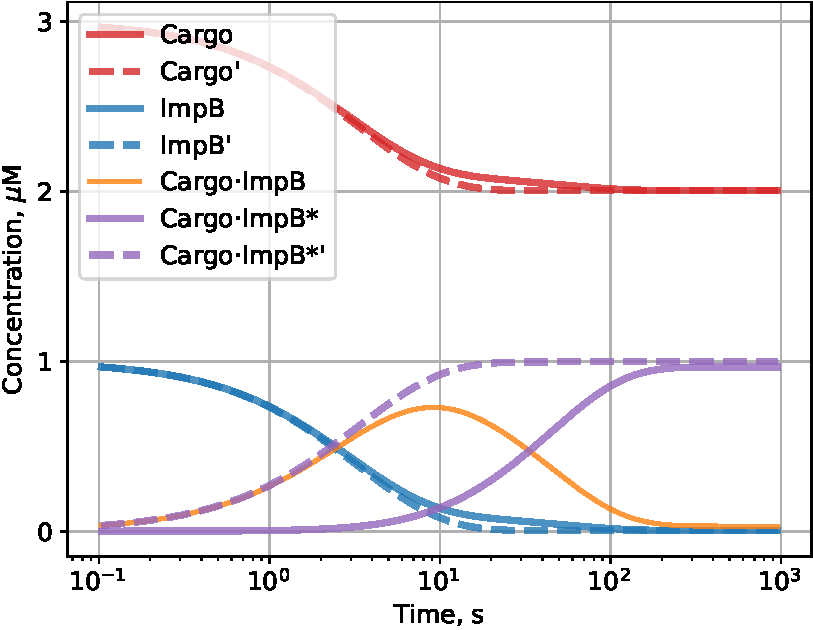
\includegraphics[width=0.5\textwidth]{20210407-Rearrangement/python/timecourse}
%\caption{%
%	Stand-alone
%	simulation of
%	\eqref{e:A*B}
%	starting with 
%	$\SI{2}{\micro M}$ \ce{IBB}
%	and
%	$\SI{1}{\micro M}$ \ce{Imp\beta}
%	with
%	the constants \eqref{e:k-A*B}.
%	%
%	The dashed counterpart
%	is the effective system 
%	of the form
%	$\ce{A} + \ce{B} \rightleftharpoons \ce{AB}$,
%	cf.~\S\ref{s:GSR03:Imp}.
%}
%\label{f:A*B}
%\end{figure}



%

With the constants from Table~\ref{t:GSR-ImpB-const},
the steady-state of the model
(reached after some $10^4 \si{. s}$)
is reported in Fig.~\ref{f:GSR-v2}.
%
Nuclear
accumulation of free cargo
is
\protect37\unskip
-fold.
%
%
Sensitivity analysis shows
that, in relative terms,
the final nuclear concentration of free cargo
depends 
most strongly
on
$k_\text{knockoff}$.
%
Doubling $k_\text{knockoff}$ almost doubles 
the nuclear concentration.
%
%
%
See Code \CODE{main/code/20210225-GSR/v2}.

%

This model predicts a slight accumulation
of \ce{Img$\upbeta$} in the nucleus,
with \ce{Imp$\upbeta$.Ran.GTP} contributing most of the excess.
%
%
%We improve on it in \S\ref{ss:3s}.

%\TODO{fluxes in Fig 1}

\begin{figure}
\centering
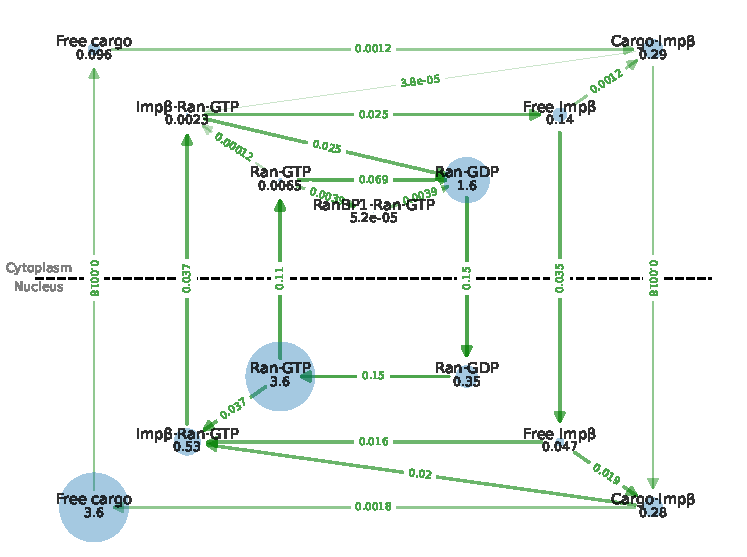
\includegraphics[width=0.7\textwidth]{20210225-GSR/v2/python/graph/onion}
\caption{%
	Steady-state of 
	the transport system from 
	\S\ref{s:GSR03:Imp}
	with conditions 
	of Table~\ref{t:GSR-ImpB-const}.
	%
	The free cargo
	shows 
	\protect37\unskip%
	-fold accumulation
	in the nucleus;
	total nuclear to total cytoplasmic cargo
	is
	\protect10\unskip%
	-fold.
	%
	Units are \si{\micro M} for species
	and \si{\micro M . s^{-1}} for fluxes.
	%
	Initial conditions:
	$[\ce{Ran . GDP}]_\text{cyt} = \SI{5}{\micro M}$,
	$[\ce{Imp\beta}]_\text{cyt} = \SI{1}{\micro M}$,
	$[\ce{Cargo}]_\text{cyt} = \SI{3}{\micro M}$,
	all else zero.
}
\label{f:GSR-v2}
\end{figure}




\begin{table}
\centering
\small
\begin{tabular}{c|c|c}
	\hline
	%
	%
	\eqref{e:v2-R}
	&
	$k_\text{on}^\text{R} = \SI{0.096}{\micro M^{-1} . s^{-1}}$,
	\;
	$k_\text{off}^\text{R} = \SI{4.8e-6}{s^{-1}}$
	&
	\footnotesize
	\cite[Supp.~Table~A]{GoerlichSeewaldRibbeck2003},
	\cite[Table II]{RiddickMacara2005}
	\\
	\hline
	%
	%
	\eqref{e:v2-C}
	&
	$k_\text{on}^\text{C} = \SI{0.11}{\micro M^{-1} . s^{-1}}$,
	\quad
	$k_\text{off}^\text{C} = \SI{7.2e-4}{s^{-1}}$
	&
	\cite[Table~I]{Catimel2001},
	\cite[Table~II]{RiddickMacara2005}
	\\
	\hline
	%
	%
	\eqref{e:knockoff}
	&
	$k_\text{knockoff} = \SI{2e-2}{\micro M^{-1} s^{-1}}$
	&
	\cite[Table II]{RiddickMacara2005}
	\\
	\hline
	%
	%
	\eqref{e:F4}
	&
	\makecell{
		$D_{\ce{Imp\beta . Ran . GTP}} = \SI{0.07}{s^{-1}}$, \quad
		$D_{\ce{Imp\beta}} = \SI{0.4}{s^{-1}}$
		\\
		$D_{\ce{Imp\beta . Cargo}} = \SI{0.25}{s^{-1}}$, \;	
		$D_{\ce{Cargo}} = \SI{5e-4}{s^{-1}}$
	}
	&
	\cite[Table III]{RiddickMacara2005}
	\\
	\hline
\end{tabular}
%
\caption{%
	Constants for the \ce{Imp$\beta$}-mediated
	transport from \S\ref{s:GSR03:Imp}.
}
%
\label{t:GSR-ImpB-const}
\end{table}



%%




\subsection{GTP hydrolysis and role of RanBP1} \label{ss:ranbp1}

According to 
\cite[\href{https://i.ibb.co/6ghqPB7/image.jpg}{Fig.~4A}]{LounsburyMacara1997},
{Imp$\upbeta$} blocks hydrolysis of {RanGTP} by {RanGAP}
but 
{RanBP1} rescues it for most part.
%
%
Similarly,
\cite{BischoffGoerlich1997}
showed that
{RanBP1} transiently detaches {Ran} 
from the complex 
Kap\ce{.}RanGTP
(where {Kap} is some karyopherin),
whereupon hydrolysis by {RanGAP} 
disassembles the complex;
and
that efficient disassembly 
of {Imp$\upbeta$}\ce{.}RanGTP required {{RanBP1}} \emph{and} {{Imp$\upalpha$}}
\cite[\S3.2, cf.~\href{https://i.ibb.co/PZKRSJ0/image.jpg}{Fig.~4}]{BischoffGoerlich1997},
\cite{FloerBlobelRexach1997}.
%
%
Importantly,
Kaps and RanBP1
bind {Ran}
at distinct sites
\cite[p.253]{BischoffGoerlich1997}.

%

%	In \cite[p.1033]{RiddickMacara2005},
%	the initial rate of cargo import
%	increased with co-addition of \ce{{RanBP1}},
%	disagreeing with their simulation
%	(in which \ce{{RanBP1}} acts catalytically
%	\cite[\href{https://i.ibb.co/B3sgJ1P/image.png}{Fig.~S1}]{RiddickMacara2005}).

%

Further,
\cite[\href{https://i.ibb.co/jz37PW1/image.png}{Fig.~13}]{SeewaldETAL2003}
characterizes
the kinetics of the formation of the complex
between
{RanGTP}, {{RanBP1}} and {RanGAP}
and the hydrolysis.
%
%
In particular, 
the release rate of the $\gamma$-phosphate,
on the order or \SI{10}{s^{-1}} in 
\cite[\href{https://i.ibb.co/jz37PW1/image.png}{Fig.~13}]{SeewaldETAL2003},
%(which is the rate-limiting step of hydrolysis by \ce{RanGAP}) % ?
is barely influenced by {{RanBP1}},
which instead stimulates
the association of {Ran} with {RanGAP}.
%
%
%
A computational model of hydrolysis
with these parameters qualitatively reproduces
the experimental data from
\cite[\href{https://i.ibb.co/6ghqPB7/image.jpg}{Fig.~4A}]{LounsburyMacara1997}.
%
%
We omit the details
that can be found in Code \protect\CODE{main/code/20210403-StickyPore/c\_rangap-sequence}.

%

For simplicity,
we will take the constant
\[
	\label{e:hydrolysis}
	%
	\text{
		{GTP} hydrolysis rate
		of \SI{0.1}{s^{-1}}
	}
\]
for all cytoplasmic-side species containing {RanGTP},
and
no {GTP} hydrolysis elsewhere.
%
%
This should be compared with 
the effective {Ran} gradient rate \eqref{e:pump}.
%
%
Reducing this rate even 1000-fold
does not substantially change the subsequent results
(not shown).

%\TODO{
%cf
%\cite{KalitaKapinosLim2021}
%citing
%\cite{KlebeBischoffPonstinglWittinghofer1995}
%or
%\cite{KlebePrinzWittinghoferGoody1995}
%}

%\begin{figure}
%\centering
%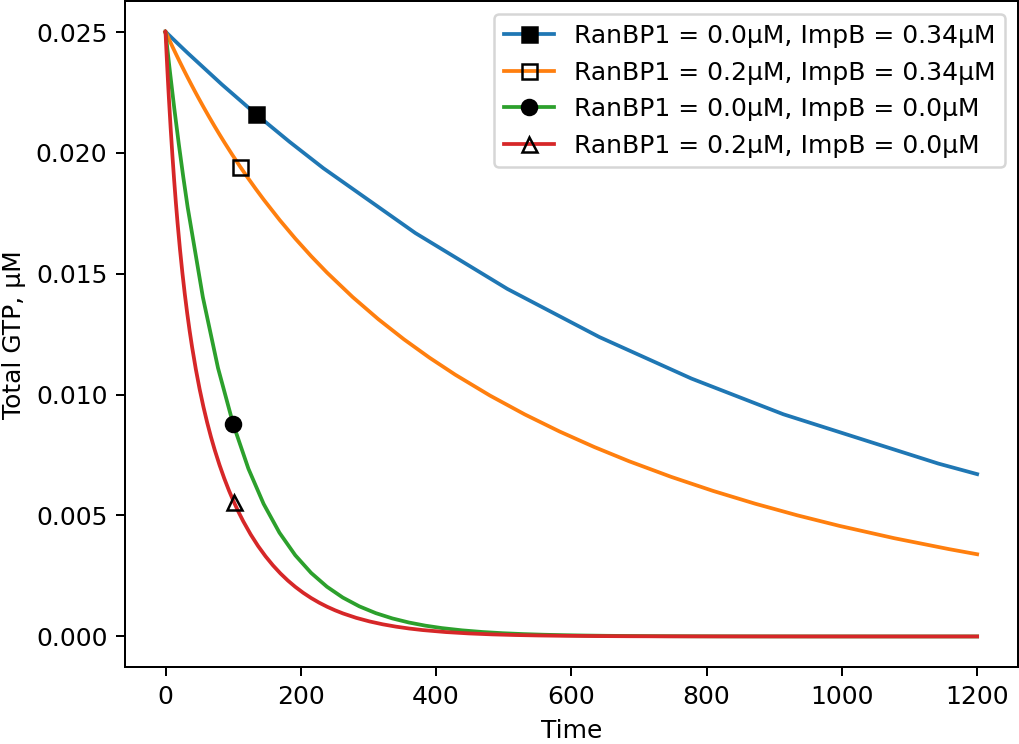
\includegraphics[width=0.7\textwidth]{20210403-StickyPore/c_rangap-sequence/python/plot_fig4a/RanGAP=0.01}
%\caption{%
%	TODO TODO
%}
%\label{f:4A}
%\end{figure}



%Notes:
%%
%Crystal structure: \cite{SaricETAL2007};
%%
%Compartments: \cite{Hofmeyr2020};
%%
%Identification of \ce{CAS}:
%\cite{KutayETAL1997}




\subsection{NPC as compartment} \label{ss:3s}

\subsubsection*{Introduction}

It has been observed,
see
\cite{KalitaKapinosLim2021} and references therein,
that Imp$\upbeta$ accumulates 
inside the NPCs
as they bind to the FG-nups (``rim staining''),
suggesting a regulatory role,
and
possibly shuttling
the cargo across the pore
repeatedly.
%
%
To account for this
we propose
a model
with cytoplasm, nucleus
and
the NPCs 
as three compartments.
%
%
The following dual observation is essential, cf.~\cite[\S10]{Hofmeyr2020}:
%
\begin{enumerate}
\item 
	cytoplasmic and nuclear species initially react 
	with NPC components in proportion
	to the number of NPCs,
	and
\item
	the observed fluorescence signal
	from Kaps accumulating inside the NPCs
	scales with
	the total volume or the capacity of the NPC channel
	(rather than their number).
\end{enumerate}

%
%
%

The model includes the following main components:
%
\begin{itemize}
\item
	\ce{Imp$\upbeta$}
	(a.k.a.~\ce{Kap$\upbeta${1}})
	and the cargo adapter
	\ce{Imp$\upalpha$}
	(a.k.a.~\ce{Kap$\upalpha$}).
	%
	For simplicity,
	we do not model individual variants/paralogs/isoforms,
	cf.~\cite[p.~2]{KalitaKapinosLim2021}.
\item
	Generic \ce{NLS} cargo,
	by itself unable to transition the nuclear envelope efficiently.
	%
	Requires the \ce{Imp$\upalpha$} adapter
	in order to be captured by \ce{Imp$\upbeta$}.
\item
	\ce{CAS}
	(a.k.a.~\ce{Exp{2}}, \ce{Xpo{2}})
	%
	Recycles \ce{Imp$\upalpha$} back to the cytoplasm.
\item
	The NPCs are described
	as
	vacant \ce{NPC} channel space,
	the cytoplasm-facing opening \ce{NPC(c)}
	and
	the nucleus-facing opening \ce{NPC(n)}.
	%
	To transition the nuclear pore,
	a species has to bind to the opening,
	transition into the channel,
	bind to the other opening,
	and unbind on the other side.
	%
	This allows us to model the capacity of the NPC
	and the dwelling time
	(but we make no distinction between different transiting species).
	%
	There is no directionality,
	i.e.~a species currently residing in the channel is equally
	likely to bind to either opening next.
\item
	\ce{Ran . GTP} in the nucleus and \ce{Ran . GDP} in the cytoplasm.
	%
	The consumption of \ce{Ran . GTP}
	that have transitioned to the cytoplasmic side
	by hydrolysis
	is compensated by an effective pump
	as in \eqref{e:pump}.
	%
	The hydrolysis itself is described by one 
	effective kinetic rate as in \eqref{e:hydrolysis}.
\end{itemize}

%

An overview of the model is shown
in Fig.~\ref{f:app:3s-simbio}.
%
The code is found in Code~\CODE{main/code/20211018-Appli}.
%
The computational results 
for this model 
are summarized in Fig.~\ref{f:app:3s-plot-ss}.
%
For details visit the URL
\newcommand{\checkpoint}{20220225-075632}
\[
	\label{e:checkpoint}
	%
	\small
	\text{
		https://numpde.github.io/nct1/code/20211018-Appli/checkpoint/%
		\href%
		{https://numpde.github.io/nct1/code/20211018-Appli/checkpoint/\checkpoint/}%
		{\checkpoint/}
	}
\]





\subsubsection*{Main reactions}

Here we comment on the main reactions of the model.
%
%
For the complete set we refer to
Fig.~\ref{f:app:3s-simbio} 
as well as the URL \eqref{e:checkpoint}.

\begin{itemize}
\item

The nuclear \ce{Ran . GTP} is converted directly to 
cytoplasmic \ce{Ran . GDP} 
as in Eqn.~\eqref{e:pump}.

\item

The \ce{Imp$\upbeta$}
can shuttle on its own through the NPC
or in complex with \ce{Imp$\upalpha$}.
%
%
We assume that the complex does not form
on the nuclear side
(due to nuclear \ce{Ran . GEF}, which is not modeled explicitly).

\item

The cytoplasmic \ce{NLS} cargo
associates with 
free cytoplasmic \ce{Imp$\upalpha$ . Imp$\upbeta$}
before binding to the cytoplasmic side of the NPC,
or
with those already attached there.
%
%
%
Once the complex is shuttled to the nuclear side,
the ``knockoff'' reaction releases the cargo
(the suffix \ce{(n)} is omitted):
\[
	\nonumber
	%
	% [Ran·GTP(n)] + [NLS·ImpA·ImpB·NPC(n)] -> [Ran·GTP·ImpB·NPC(n)] + [ImpA(n)] + [NLS(n)]
	\ce{
		Ran.GTP
		+
		NLS.Imp$\upalpha$.Imp$\upbeta$.NPC
		->
		Ran.GTP.Imp$\upbeta$.NPC
		+
		Imp$\upalpha$
		+
		NLS
	}
	.
\]
%
%
Thereupon, the complex \ce{Ran . GTP . Imp$\upbeta$}
can transition from the nuclear to the cytoplasmic side
to be hydrolized as in Eqn.~\eqref{e:hydrolysis}.

\item

Like \ce{Imp$\upbeta$},
\ce{CAS} can shuttle through the NPC.
%
%
On the nuclear side,
it first binds to \ce{Ran . GTP}
then
forms
the \ce{Imp$\upalpha$ . CAS . Ran . GTP} complex,
%
which can shuttle through the NPC,
and is disassembled
on the cytoplasmic side
by the hydrolysis reaction \eqref{e:hydrolysis}.

\end{itemize}


\subsubsection*{Baseline parameters} \label{ss:3s:baseline}

Here we comment on the choice of 
selected
model parameters,
such as concentrations and kinetic rates.
%
%
For the complete set 
see the URL \eqref{e:checkpoint}.

\begin{itemize}

\item

The nucleus and the cytoplasm each have a volume
of \SI{1}{\pico L}.


\item

We estimate the total NPC channel capacity
as 
2000 NPCs per nuclear envelope
[BioNumbers, \href{https://bionumbers.hms.harvard.edu/bionumber.aspx?id=111130}{\#111130}]
times
300 Kaps per NPC
\cite[\href{https://i.ibb.co/8jdLvn1/Paradise-Levin-Korza-Carson-2007-Fig7.jpg}{Fig.~7}]{ParadiseETAL2007}.
%
%
Note that 
$ %\[
	%\label{e:NPC-volume}
	%
	\SI{1}{\micro M} \times \SI{1}{\pico L} 
	\approx
	300 \times \SI{2000}{units}
	,	
$ %\]
which implies a concentration of \SI{1}{\micro M}
in a computational volume of \SI{1}{\pico L}.
%
%
%
The computation itself is performed in amounts
(not concentration),
so to convert to apparent concentration
of Kaps at the NE
we estimate
the volume of the NE as \SI{0.01}{\pico L}.
%
This only scales
the concentrations 
shown in the figures.


\item

For the initial concentration of \ce{Imp$\upbeta$}
we take
\SI{5}{\micro M}
in nucleus and cytoplasm
based on
\cite[\href{https://i.ibb.co/1mNP2XT/Kalita-Kapinos-Lim2021-Fig4.png}{Fig.~4}]{KalitaKapinosLim2021} / 
\cite[\href{https://i.ibb.co/0nLsTZv/Screenshot-from-2022-01-28-15-03-10.png}{Fig.~4a}]{NguyenPappireddiWuhr2019}.
%
% -- probably from \cite{WuhrETAL2014}

% \cite{YangMusser2006}


\item

For the initial concentration of \ce{Imp$\upalpha$}
we considered 
\SI{5}{\micro M} throughout the cell
based on
%
the immunoblots of
\cite[\href{https://i.ibb.co/1z0YJ0T/Screenshot-from-2022-01-28-10-49-23.png}{Fig.~7}]{ZienkiewiczETAL2013}
%
and the mass spectrometry measurements for 
\href{https://www.genecards.org/Search/Symbol?queryString=KPNA*}{KPNAs}
from
\cite[Table~S5]{WuhrETAL2014}.
%
This corresponds to all variants of Kap$\upalpha$ (KPNA2,3,4,6).
%
%
However,
this seemed incompatible with other parameters,
%in that the steady state showed unexpected results,
e.g.~%
the NLS remained tied to {Imp$\upalpha$}
and nearly equal at nuclear and cytoplasmic sides.
%
%
We settled on the {Imp$\upalpha$} concentration of \SI{0.5}{\micro M}
for the baseline model,
which is close to the previously reported concentration
of the single Kap$\upalpha$1 (\href{https://www.genecards.org/cgi-bin/carddisp.pl?gene=KPNA2}{KPNA2}).

%\cite{KalitaKapinosLim2021}
%\cite{KirliETAL2015}

\end{itemize}

  
Simulating this scenario
we observe
\begin{itemize}
\item 
	strong accumulation of NLS cargo
	in the nucleus,
	most of it free;
\item
	no N:C contrast for Imp$\upbeta$,
	with some accumulation at the nuclear envelope;
\item
	a N:C contrast of 3:1 for Imp$\upalpha$,
	almost all of it bound;
\item
	a N:C contrast of about 4:1 for free CAS
	and 4:3 for all CAS;
\item
	about 70\% of initial RanGTP
	unbound in the nucleus.
\end{itemize}



%

\subsubsection*{Variants}

We define a handful of scenarios 
to illustrate how 
parameter choice affects 
the steady-states.
%
These changes could mimic
different cell types, disease
or
configurations of the artificial cell.
%
They can be generated in vivo
by depletion (e.g.~via siRNA)
or 
by transfection with a vector overexpressing a protein.
%
%
The results are summarized in Fig.~\ref{f:app:3s-plot-ss}.
%
%
All parameter changes are
with respected 
to the baseline scenario,
and are documented in full at the URL \eqref{e:checkpoint}.
%
%
%
We expect the artificial cell 
to reproduce those trends.



\begin{enumerate}
\item 
	Decrease \ce{Imp$\upbeta$} 10x.
	%
	We observe a higher N:C contrast of cargo and of Imp$\upalpha$.
	
\item
	Increase the number of NPCs 10x.
	%
	More transport receptors are now bound to the NPC,
	thus exhibiting a higher concentration
 	at the nuclear envelope, cf.~\cite{KalitaETAL2022}.
	
\item
	Increase \ce{Imp$\upalpha$} 10x.
	%
	We observe a breakdown of transport.

\item
	Decrease \ce{Imp$\upalpha$} 10x.
	%
	Leads to enhanced N:C contrasts
	of CAS, Imp$\upalpha$ and NLS cargo.
	
\item
	Turn off \ce{Ran.GTP} regeneration,
	starting from the baseline scenario.
	%
	%
	We obtain a breakdown of N:C contrast
	for all species,
	as expected.
\end{enumerate}



\begin{figure} %[!p]
	\centering
	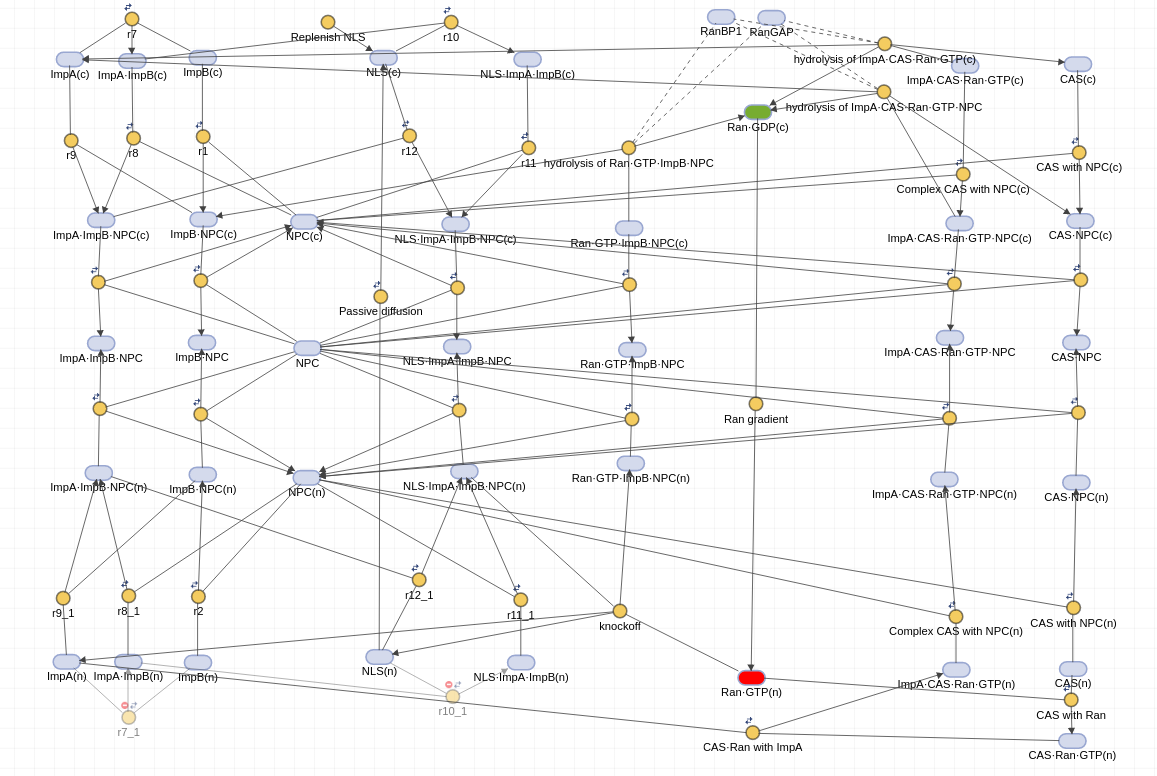
\includegraphics[width=0.95\textwidth]{20211018-Appli/threestage}
	\caption{%
		SimBiology diagram for the model 
		``\nameref{ss:3s}'' from \S\ref{ss:3s}.
		%
		%
		The ovals represent chemical species,
		the yellow circles are reactions
		(some are reversible).
		%
		%
		The middle row (containing free NPC)
		are species inside the NPC.
		%
		%
		The row above and below are species
		bound to 
		the cytoplasmic-side and nuclear-side 
		of the NPCs, respectively.
		%
		%
		The top row are cytoplasmic species
		and
		the bottom row are nuclear species.  
	}
	\label{f:app:3s-simbio}
\end{figure}


\clearpage
\thispagestyle{empty}

\begin{figure}[!h]

	\centering
	
	\newcommand{\figpath}{20211018-Appli/checkpoint/\checkpoint/plot_ss}
	\newcommand{\figures}{\fig{Free ImpA}\\\fig{Free ImpB}\\\fig{Free CAS}\\\fig{Free NLS}}
	
	\begin{minipage}{0.49\textwidth}
		\centering
		%
		Baseline \\[0.5\baselineskip]
		%
		\newcommand\fig[1]{\includegraphics[width=\textwidth]{\figpath/a_Baseline/#1}}
		\figures
	\end{minipage}
	%
	\hfill
	%
	\begin{minipage}{0.49\textwidth}
		\centering
		%
		Decrease \ce{Imp$\upbeta$} \\[0.5\baselineskip]
		%
		\newcommand\fig[1]{\includegraphics[width=\textwidth]{\figpath/b_LowImpB/#1}}
		\figures
	\end{minipage}
	
	\vspace{\baselineskip}
	
	\begin{minipage}{0.49\textwidth}
		\centering
		%
		Increase NPC \\[0.5\baselineskip]
		%
		\newcommand\fig[1]{\includegraphics[width=\textwidth]{\figpath/c_MoreNPC/#1}}
		\figures
	\end{minipage}
	%
	\hfill
	%
	\begin{minipage}{0.49\textwidth}
		\centering
		%
		Increase \ce{Imp$\upalpha$} \\[0.5\baselineskip]
		%
		\newcommand\fig[1]{\includegraphics[width=\textwidth]{\figpath/d_HighImpA/#1}}
		\figures
	\end{minipage}
	
	\vspace{\baselineskip}
	
	\begin{minipage}{0.49\textwidth}
		\centering
		%
		Decrease \ce{Imp$\upalpha$} \\[0.5\baselineskip]
		%
		\newcommand\fig[1]{\includegraphics[width=\textwidth]{\figpath/d_LowImpA/#1}}
		\figures
	\end{minipage}
	%
	\hfill
	%
	\begin{minipage}{0.49\textwidth}
		\centering
		%
		No \ce{Ran.GTP} regeneration \\[0.5\baselineskip]
		%
		\newcommand\fig[1]{\includegraphics[width=\textwidth]{\figpath/e_NoEnergy/#1}}
		\figures
	\end{minipage}
	
	\vspace{\baselineskip}
		
	\caption{%
		Initial states and final steady-states for the model 
		``\nameref{ss:3s}'' from \S\ref{ss:3s}
		at the cytoplasmic side (c),
		inside the NPCs (NPC)
		and 
		at the nuclear side (n),
		for 
		free ImpA, free ImpB, free CAS and free NLS cargo.
		%
		%
		%
		For full-size figures and time-course plots, see the URL \eqref{e:checkpoint}.
	}
	%
	\label{f:app:3s-plot-ss}
\end{figure}




%\section{Conclusions}
%
%\TODO{conclude}



%%% BIBLIOGRAPHY %%%

\clearpage

\renewcommand*{\bibfont}{\normalfont\small}
\printbibliography % biblatex


\section*{List of codes}

\begin{center}
\SHOWCODES
\end{center}



`\clearpage

\section{Appendix: minimal Ran gradient system} \label{s:app:gsr-ran}



Here we recapitulate
the minimal Ran gradient system
from \cite[Fig.~2]{GoerlichSeewaldRibbeck2003},
cf.~\S\ref{s:GSR03}.
%
%
The following account for the cytoplasmic species.
%
Here,
$\ce{[\ldots]}$ abbreviates 
the (cytoplasmic) concentration of 
the complex \ce{{RanBP1} . Ran.GTP}.
%(in presence of \ce{RanGAP}, this term can be omitted).
%
\ce{Ex} is an additional potentially useful flux of 
nuclear \ce{Ran.GTP} to cytoplasmic \ce{Ran.GDP},
set by default to zero.
%
%
\begin{subequations}
\small
\[
	\label{e:Eq1}
	%
	\ddt
	[\ce{Ran.GDP}]_\text{cyt}
	& =
	\ce{F_{\ce{Ran.GDP}}} \frac{V_\text{nuc}}{V_\text{cyt}} 
	+
	\ce{GAP}
	+
	\ce{GAP_{RanBP1}}
	+
	\ce{Ex} \frac{V_\text{nuc}}{V_\text{cyt}} 
	%
	%
	\\
	\label{e:Eq2}
	%
	\ddt
	[\ce{Ran.GTP}]_\text{cyt}
	& = 
	\ce{F_{\ce{Ran.GTP}}} \frac{V_\text{nuc}}{V_\text{cyt}}
	-
	\ce{GAP}
	-
	k_\text{on}^\text{rbp}
	[\ce{{RanBP1}}] [\ce{Ran.GTP}]_\text{cyt}
	+
	k_\text{off}^\text{rbp}
	[\ce{\ldots}]
	%
	%
	\\
	\label{e:Eq3}
	%
	\ddt
	[\ce{{RanBP1} . Ran.GTP}]
	& =
	-
	\ce{GAP_{RanBP1}}
	\quad\quad\quad
	+
	k_\text{on}^\text{rbp}
	[\ce{{RanBP1}}] [\ce{Ran.GTP}]_\text{cyt}
	-
	k_\text{off}^\text{rbp}
	[\ce{\ldots}]
\]
\end{subequations}
%
%
The following account for the nuclear species.
%
As in \cite{GoerlichSeewaldRibbeck2003},
\ce{E} denotes free \ce{{RCC1}}.
%
%
\begin{subequations}
\[
	\label{e:Eq4}
	%
	\ddt
	[\ce{Ran.GDP}]_\text{nuc}
	& =
	-
	\ce{F_{\ce{Ran.GDP}}}
	+
	r_8
	[\ce{IntC}]
	-
	r_1
	[\ce{E}]
	[\ce{Ran.GDP}]_\text{nuc}
	%
	%
	\\
	\label{e:Eq5}
	%
	\ddt
	[\ce{Ran.GTP}]_\text{nuc}
	& =
	-
	\ce{F_{\ce{Ran.GTP}}}
	+
	r_4
	[\ce{IntA}]
	-
	r_5
	[\ce{E}]
	[\ce{Ran.GTP}]_\text{nuc}
	-
	\ce{Ex}
\]
\end{subequations}
%
%
The nucleotide-exchange reaction
\ce{Ran.GDP + GTP <=> Ran.GTP + GDP}
is catalyzed by \ce{{RCC1}}.
%
It is modeled as in 
\cite[Fig.~6]{KlebePrinzWittinghoferGoody1995}
/
\cite[Fig.~1]{GoerlichSeewaldRibbeck2003}
with three intermediates.
%
Note that it depends on
the availability of \ce{GDP} and \ce{GTP}.
%
%
\begin{subequations}
\[
	\label{e:Eq6}
	%
	\ddt
	[\ce{IntA}]
	& =
	-(r_4 + r_6)
	[\ce{IntA}]
	+
	r_5
	[\ce{E}] [\ce{Ran.GTP}]_\text{nuc}
	+
	r_3
	[\ce{GTP}] [\ce{IntB}]
	%
	%
	\\
	\label{e:Eq7}
	%
	%
	\ddt
	[\ce{IntB}]
	& =
	r_6 [\ce{IntA}]
	+
	r_2 [\ce{IntC}]
	-
	(r_3 [\ce{GTP}] + r_7 [\ce{GDP}])
	[\ce{IntB}]
	%
	\\
	\label{e:Eq8}
	%
	\ddt
	[\ce{IntC}]
	& =
	-
	(r_2 + r_8) [\ce{IntC}]
	+
	r_1 [\ce{E}] [\ce{Ran.GDP}]_\text{nuc}
	+
	r_7 [\ce{GDP}] [\ce{IntB}]
\]
\end{subequations}
%
%
Constraints on the total concentration:
%
%
\begin{subequations}
\[
	\label{e:Eq9}
	%
	\text{Free \ce{{RCC1}}}:
	& &
	\ce{[E]}
	& =
	\ce{{RCC1}_{total}} - (\ce{[IntA]} + \ce{[IntB]} + \ce{[IntC]})
	%
	\\
	\label{e:Eq10}
	%
	\text{Free \ce{{RanBP1}}}:
	& &
	\ce{[{RanBP1}]}
	& =
	\ce{{RanBP1}_{total}} - \ce{[{RanBP1} . Ran.GTP]}
\]
\end{subequations}
%
%
Gradient-driven fluxes from 
the nucleus to the cytoplasm:
%
%
\begin{subequations}
\[
	\label{e:Eq11}
	%
	\ce{F_{Ran.GTP}}
	& =
	D_{\ce{Ran.GTP}}
	\;
	([\ce{Ran.GTP}]_\text{nuc} - [\ce{Ran.GTP}]_\text{cyt})
	%
	\\
	\label{e:Eq12}
	%
	\ce{F_{Ran.GDP}}
	& =
	D_{\ce{Ran.GDP}}
	\;
	([\ce{Ran.GDP}]_\text{nuc} - [\ce{Ran.GDP}]_\text{cyt})
\]
\end{subequations}
%
%
\ce{RanGAP} hydrolyzes the $\gamma$-phosphate of \ce{Ran.GTP}.
%
This is more efficient
when \ce{Ran.GTP} is bound to \ce{{RanBP1}}
\cite{BischoffKrebberSmirnovaDongPonstingl1995},
reducing the IC50 seven-fold
\cite[Table~I, p.~1091]{GoerlichSeewaldRibbeck2003}.
%
%
%
\begin{subequations}
\[
	\label{e:Eq13}
	%
	\ce{GAP} 
	& = 
	k_{\ce{GAP}} [\ce{RanGAP}]
	/
	(
		1 + K_{\ce{GAP}} / [\ce{Ran.GTP}]_\text{cyt}
	)
	%
	\\
	\label{e:Eq14}
	%
	\ce{GAP_{RanBP1}} 
	& = 
	k_{\ce{GAP}}' [\ce{RanGAP}]
	/
	(
		1 + K_{\ce{GAP}}' / [\ce{{RanBP1} . Ran.GTP}]
	)
\]
\end{subequations}
%
To determine the dynamic capacity \ce{Ex}
at steady-state
we introduce
the additional equation:
\[
	\label{e:Ex}
	%
	\ddt \ce{Ex}
	=
	k_{\ce{Ex}} \, [\ce{Ran . {GTP}}]_\text{nuc},
	\quad
	k_{\ce{Ex}} := \SI{10}{s^{-2}},
	\TEXT{initial}
	\ce{Ex} := \SI{0}{\micro M . s^{-1}}
	.
\]





\begin{table}
\centering
\small
\begin{tabular}{c|c|c}
%	Eqn & Constants & References
%	\\
	\hline
	%
	%
	\eqref{e:Eq1}
	&
	$V_\text{nuc} = \SI{1.2}{pl}$,
	\quad
	$V_\text{cyt} = \SI{1.8}{pl}$
	& 
	\cite[Table II]{GoerlichSeewaldRibbeck2003}
	\\
	\hline
	%
	%
	\eqref{e:Eq1}
	&
	initial condition
	$[\ce{Ran . GDP}]_\text{cyt} = \SI{5}{\micro M}$
	&
	\cite[Table II]{GoerlichSeewaldRibbeck2003}
	\\
	\hline
	%
	%
	\eqref{e:Eq2}--\eqref{e:Eq3}
	&
	$k_\text{on}^\text{rbp} = \SI{0.3}{\micro M^{-1}.s^{-1}}$,
	\quad
	$k_\text{off}^\text{rbp} = \SI{4e-4}{s^{-1}}$
	&
	\cite[Supp.~Table~A]{GoerlichSeewaldRibbeck2003}
	\\
	\hline
	%
	%
	\eqref{e:Eq4}--\eqref{e:Eq8}
	&
	\makecell{
		$r_1 = \SI{74}{\micro M^{-1} . s^{-1}}$,
		\quad
		$r_8 = \SI{55}{s^{-1}}$
		\\
		$r_7 = \SI{11}{\micro M^{-1} . s^{-1}}$,
		\quad
		$r_2 = \SI{21}{s^{-1}}$
		\\
		$r_3 = \SI{0.6}{\micro M^{-1} . s^{-1}}$,
		\quad
		$r_6 = \SI{19}{s^{-1}}$
		\\
		$r_5 = \SI{100}{\micro M^{-1} . s^{-1}}$,
		\quad
		$r_4 = \SI{55}{s^{-1}}$
	}
	&
	\makecell{
		\cite[Supp.~Table~A]{GoerlichSeewaldRibbeck2003}
		\\
		\cite[Fig.~6]{KlebePrinzWittinghoferGoody1995}
	}
	\\
	\hline
	%
	%
	\eqref{e:Eq6}--\eqref{e:Eq8}
	&
	$[\ce{GTP}] = \SI{500}{\micro M}$,
	\quad
	$[\ce{GDP}] = \SI{1.6}{\micro M}$
	&
	\cite[Table II]{GoerlichSeewaldRibbeck2003}
	\\
	\hline
	%
	%
	\makecell{
		\eqref{e:Eq9} \\ \eqref{e:Eq10}
	}
	&
	\makecell{
		$\ce{{RCC1}_{total}} = \SI{0.7}{\micro M}$
		\\
		$\ce{{RanBP1}_{total}} = \SI{2}{\micro M}$
	}
	&
	\makecell{
		\cite[Supp.~Table~B]{GoerlichSeewaldRibbeck2003}
		\\
		\cite[Fig.~4]{GoerlichSeewaldRibbeck2003}
	}
	\\
	\hline
	%
	%
	\makecell{
		\eqref{e:Eq11} \\ \eqref{e:Eq12}
	}
	&
	\makecell{
		$D_{\ce{Ran . GTP}} = \SI{0.03}{s^{-1}}$
		\\
		$D_{\ce{Ran . GDP}} = \SI{0.12}{s^{-1}}$
	}
	&
	\cite[Table II]{GoerlichSeewaldRibbeck2003}
	\\
	\hline
	%
	%
	\makecell{
		\eqref{e:Eq13} \\ \eqref{e:Eq14}
	}
	&
	\makecell{
		$k_{\ce{GAP}} = \SI{10.6}{s^{-1}}$,
		\quad
		$K_{\ce{GAP}} = \SI{0.7}{\micro M}$
		\\
		$k_{\ce{GAP}}' = \SI{10.8}{s^{-1}}$,
		\quad
		$K_{\ce{GAP}}' = \SI{0.1}{\micro M}$
	}
	&
	\makecell{
		\cite[Supp.~Table~A]{GoerlichSeewaldRibbeck2003}
		\\
		\cite[Table~I]{GoerlichSeewaldRibbeck2003}
	}
	\\
	\hline
	%
	%
	\eqref{e:Eq13}--\eqref{e:Eq14}
	&
	cytoplasmic
	$[\ce{RanGAP}] = \SI{0.7}{\micro M}$
	&
	\cite[Table~II / ST~B]{GoerlichSeewaldRibbeck2003}
	% / \cite[Fig.~4]{GoerlichSeewaldRibbeck2003}
	\\
	\hline
%	%
%	%
%	\TODO{Eq}
%	&
%	$K_R = \SI{5e-4}{\micro M}$
%	&
%	\cite[Supp.~Table~A]{GoerlichSeewaldRibbeck2003}
%	\\
%	\hline
\end{tabular}
%
\caption{%
	Constants
	for the ``standard simulation condition''
	of \S\ref{s:GSR03}
	at $\SI{25}{\celsius}$.
	%
	Except for \eqref{e:Eq1},
	all species are initialized to zero at $t = 0$.
}
%
\label{t:GSR-const}
\end{table}




\begin{table}
\centering
\footnotesize
\begin{tabular}{c|c|c|c|c}
	\hline
	%
	Condition
	& 
	\makecell{Affected \\ parameters}
	&
	\makecell{Nuclear \\ RanGTP, \si{\micro M}}
	&
	\makecell{Cytoplasmic \\ RanGTP, \si{\nano M}}
	&
	\makecell{Dynamic \\ capacity, \si{\micro M \per s}}
	%
	\\
	\hline\hline
	%
	``Standard''
	& 
	See Table~\ref{t:GSR-const} 
	&
	4.26
	(4.3)
	&
	7.75
	(7.7)
	&
	0.59 (0.60)
	%
	\\
	\hline
	%
	Omission of RanBP1
	&
	$\ce{{RanBP1}_{total}} := 0$
	&
	4.27
	(4.3)
	& 
	8.13
	(8.1)
	&
	0.59 (0.60)
	%
	\\
	\hline
	%
	200\% RCC1
	&
	\ce{{RCC1}_{total}}
	&
	3.95
	(4.0)
	& 
	7.17
	(7.1)
	&
	0.59 (0.60)
	%
	\\
	\hline
	%
	50\% RCC1
	&
	\ce{{RCC1}_{total}}
	&
	4.31
	(4.3)
	& 
	7.82
	(7.7)
	&
	0.58 (0.60)
	%
	\\
	\hline
	%
	10\% RCC1
	&
	\ce{{RCC1}_{total}}
	&
	3.59
	(3.6)
	& 
	6.50
	(6.4)
	&
	0.46 (0.48)
	%
	\\
	\hline
	%
	1\% RCC1
	&
	\ce{{RCC1}_{total}}
	&
	1.40
	(1.4)
	& 
	2.52
	(2.5)
	&
	0.075 (0.08)
	%
	\\
	\hline
	%
	GTP:GDP = 500:0
	&
	$[\ce{GDP}] := \SI{0}{\micro M}$
	&
	4.80
	(4.8)
	& 
	8.72
	(8.6)
	&
	0.59 (0.60)
	%
	\\
	\hline
	%
	GTP:GDP = 500:50
	&
	$[\ce{GDP}] := \frac{1}{10} [\ce{GTP}]$
	&
	0.98
	(0.8)
	& 
	1.76
	(1.5)
	&
	0.57 (0.58)
	%
	\\
	\hline
	%
	GTP:GDP = 500:500
	&
	$[\ce{GDP}] := [\ce{GTP}]$
	&
	0.12
	(0.12)
	& 
	0.22
	(0.21)
	&
	0.34 (0.34)
	%
	\\
	\hline
	%
	Saturating NTF2
	% Fig.~3
	&
	$D_{\ce{Ran . GDP}} := \SI{0.48}{s^{-1}}$
	&
	5.12
	(5.1)
	& 
	9.32
	(9.2)
	&
	2.18 (2.2)
	%
	\\
	\hline
	%
	No NTF2
	&
	$D_{\ce{Ran . GDP}} := D_{\ce{Ran . GTP}}$
	&
	2.55
	(2.5)
	& 
	4.60
	(4.5)
	&
	0.15 (0.16)
	%
	\\
	\hline
	%
	200\% RanGAP
	&
	$[\ce{RanGAP}]$
	&
	4.27
	(4.3)
	& 
	3.95
	(3.9)
	&
	0.59 (0.60)
	%
	\\
	\hline
	%
	50\% RanGAP
	&
	$[\ce{RanGAP}]$
	&
	4.26
	(4.3)
	& 
	14.9
	(14)
	&
	0.59 (0.60)
	%
	\\
	\hline
	%
	50\% permeability
	&
	$D_{\ce{Ran . GTP}}$
	&
	4.91
	(4.9)
	& 
	4.44
	(4.4)
	&
	0.59 (--)
	%
	\\
	\hline
	%
	200\% permeability
	&
	$D_{\ce{Ran . GTP}}$
	&
	3.41
	(3.4)
	& 
	12.4
	(12.3)
	&
	0.59 (--)
	%
	\\
	\hline
	%
	400\% permeability
	&
	$D_{\ce{Ran . GTP}}$
	&
	2.46
	(2.5)
	& 
	18.0
	(17.8)
	&
	0.59 (--)
	%
	\\
	\hline
\end{tabular}
\caption{%
	Steady-state concentrations
	for the simulation scenarios
	from \cite[Table~II/III]{GoerlichSeewaldRibbeck2003},
	with
	their results shown in brackets.
	%
	Value for $D_{\ce{Ran . GDP}}$ is
	from \cite[Fig.~3]{GoerlichSeewaldRibbeck2003}.
}
\label{t:GSR-Ran-Runs}
\end{table}





%\clearpage
%
%\section{TODO}
%\SHOWTODOS



\end{document}
